\section{Methodology}

The LuminaBP framework orchestrates a multi-stage pipeline designed to transition from raw facial video streams to precise arterial blood pressure estimates.

\begin{figure}[ht]
\centering
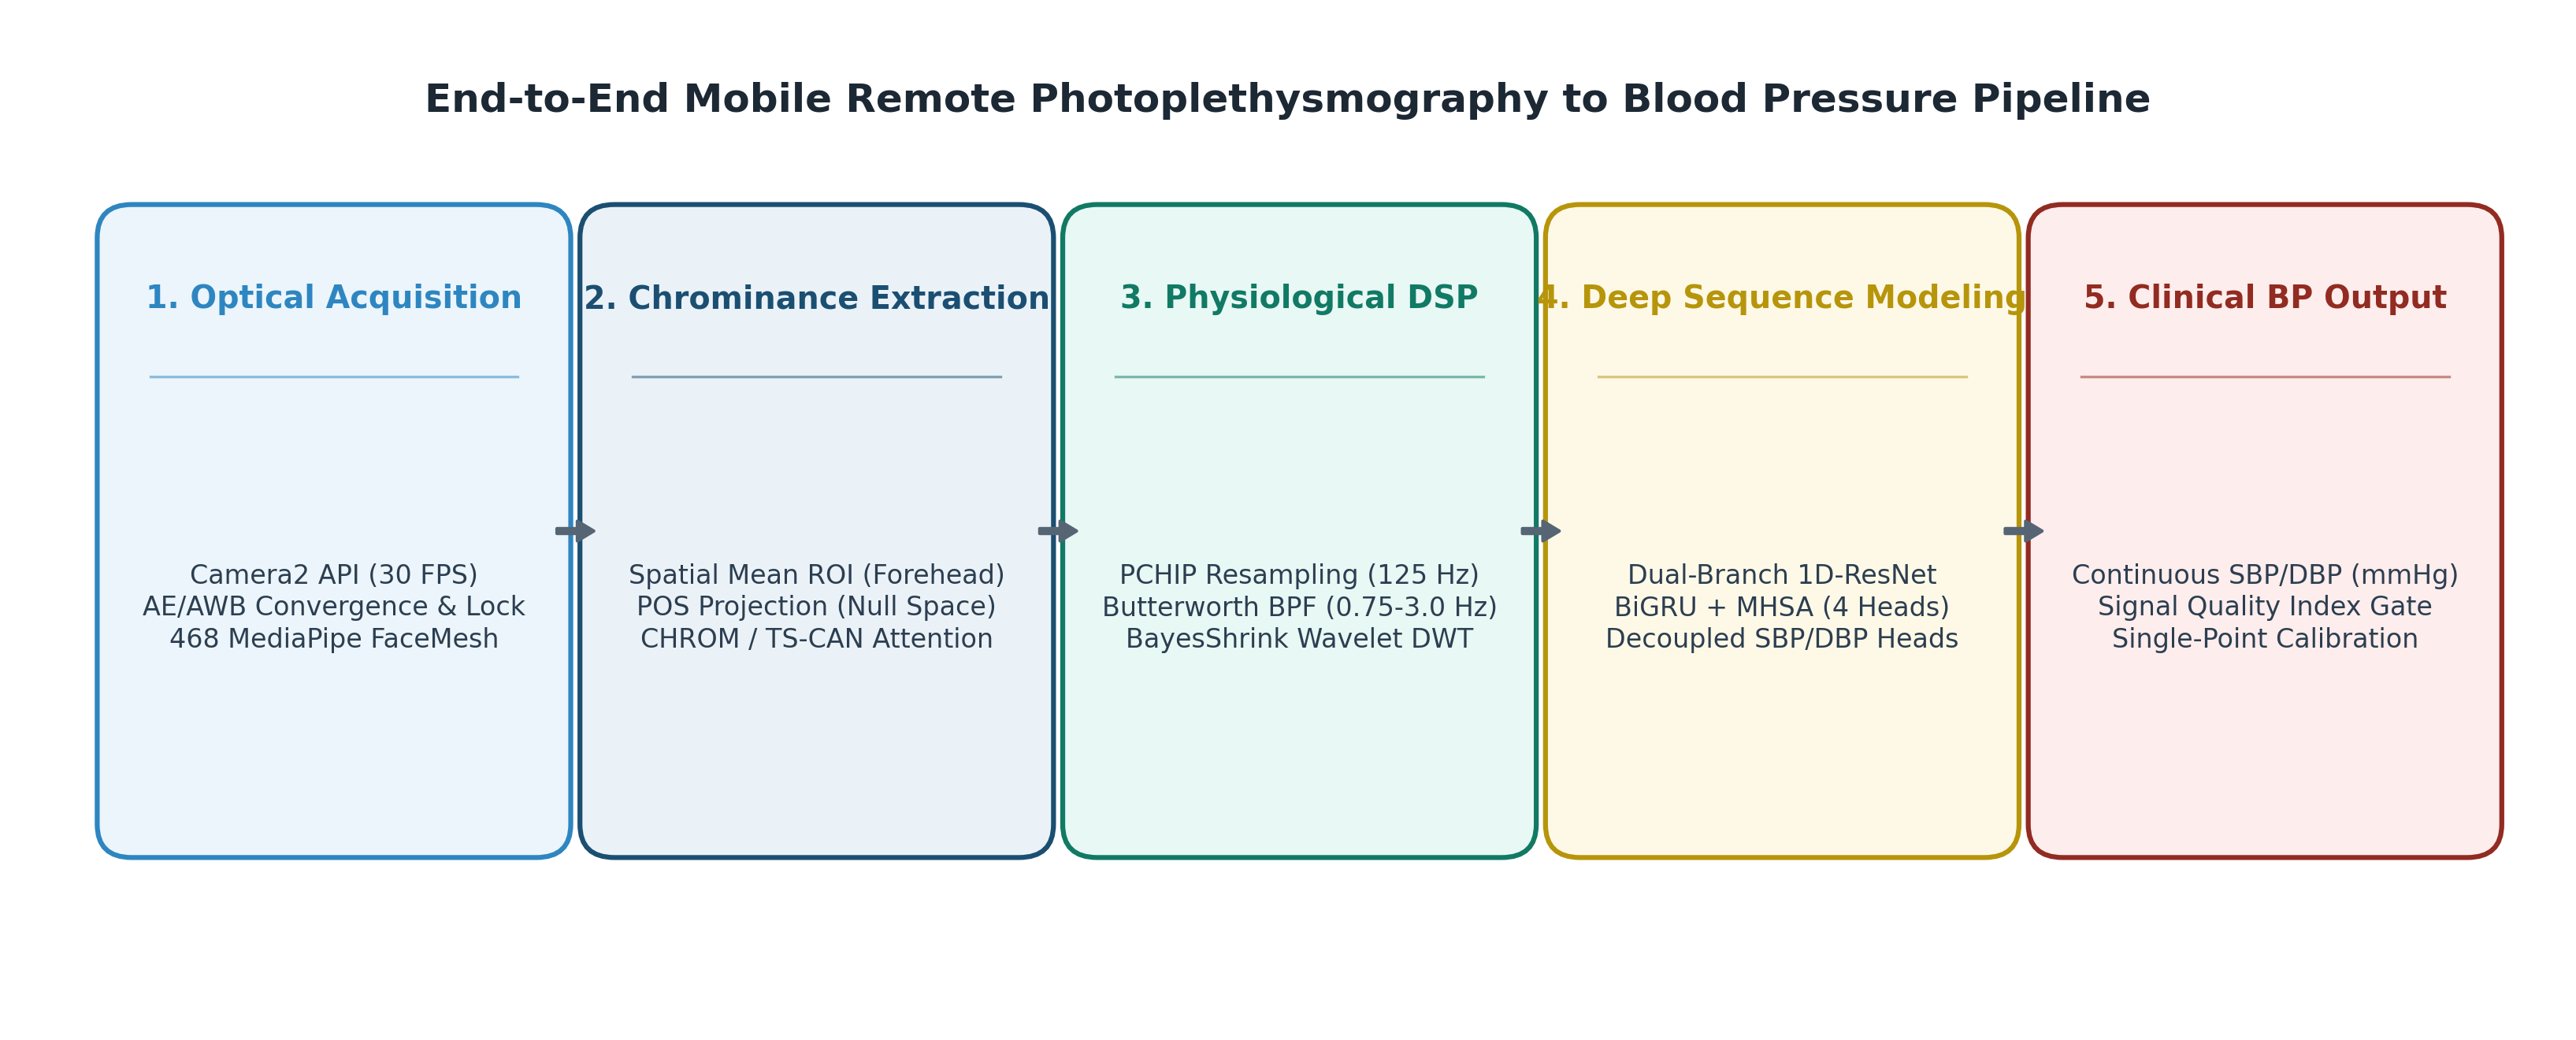
\includegraphics[width=\linewidth]{results/figures/fig_pipeline_overview.png}
\caption{End-to-End LuminaBP Pipeline Architecture: Demonstrating the transition from video acquisition, 468-point mesh tracking, POS projection, to the decoupled MODEL-06-SepHead neural network.}
\label{fig:pipeline}
\end{figure}

\subsection{Optical Signal Acquisition and Processing}
The acquisition module captures 30 FPS video with sensor-level exposure and white-balance locked to minimize non-physiological illumination jumps. Facial regions of interest (ROIs)—specifically the bilateral malar (cheek) and upper forehead regions—are tracked dynamically using a 468-point 3D MediaPipe mesh, ensuring spatial consistency even during micro-expressions or rigid head motion.

\begin{figure}[ht]
\centering
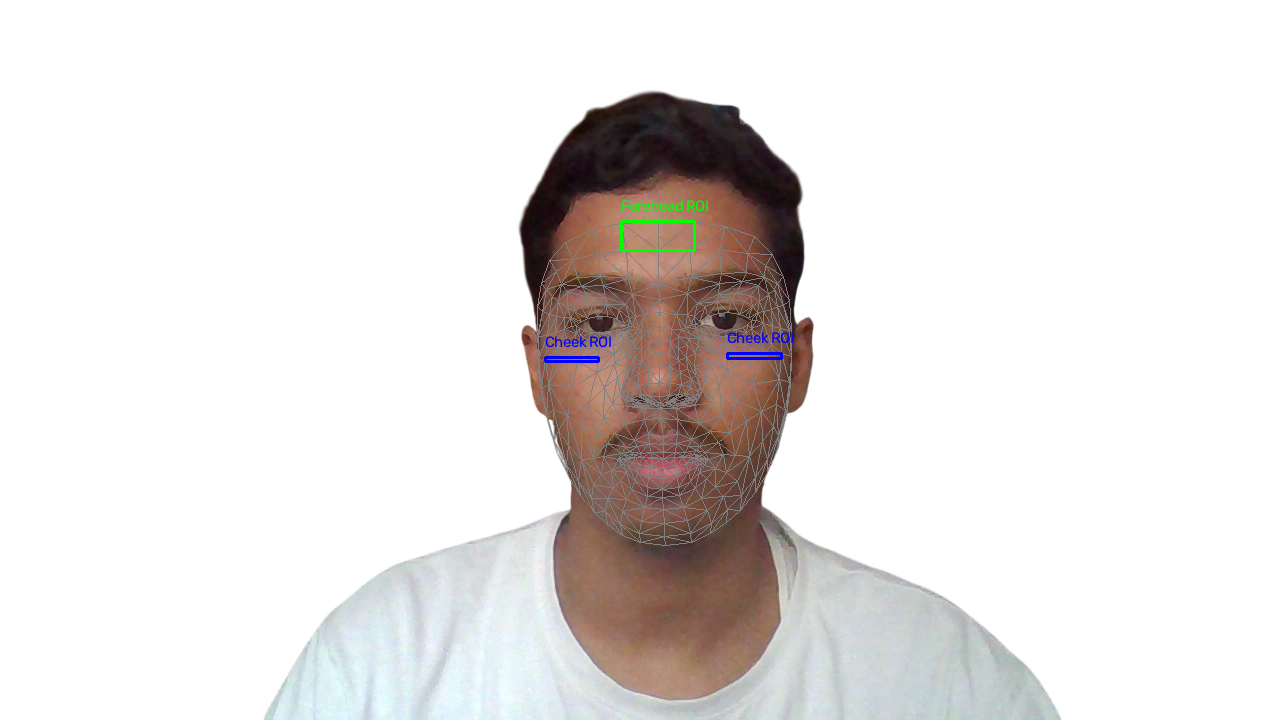
\includegraphics[width=0.7\linewidth]{results/figures/fig1_roi_wireframe.png}
\caption{Facial Region of Interest (ROI) extraction using the 468-point MediaPipe mesh. The malar and upper forehead regions exhibit optimal microvascular density.}
\label{fig:roi}
\end{figure}

The raw spatial averages from the RGB channels form the temporal signal matrix $\mathbf{C}(t) = [R(t), G(t), B(t)]^T$. We project this matrix into a 1D pulsatile signal using the POS algorithm. POS operates by defining two orthogonal projection axes on the normalized color space to eliminate the specular reflection component:
\begin{equation}
\mathbf{X}_1(t) = G(t) - B(t), \quad \mathbf{X}_2(t) = R(t) - G(t) + R(t) - B(t)
\end{equation}
The final pulse signal $h(t)$ is derived via an alpha-tuned combination:
\begin{equation}
h(t) = \mathbf{X}_1(t) + \frac{\sigma(\mathbf{X}_1)}{\sigma(\mathbf{X}_2)} \mathbf{X}_2(t)
\end{equation}

To suppress 8-bit quantization noise while strictly preserving high-order waveform derivatives (such as the dicrotic notch), we introduce an adaptive Savitzky-Golay polynomial smoothing filter in combination with a Butterworth bandpass filter (0.7--3.5 Hz).
Mathematically, the smoothed output $g_i$ is computed via local polynomial convolution:
\begin{equation}
g_i = \sum_{n = -m}^{m} c_n \cdot x_{i+n}
\end{equation}
where $c_n$ represents the least-squares polynomial coefficients over a moving window of size $2m+1$. This is vastly superior to standard moving averages or low-pass IIR filters that destroy the high-frequency dicrotic components.

\begin{figure}[ht]
\centering
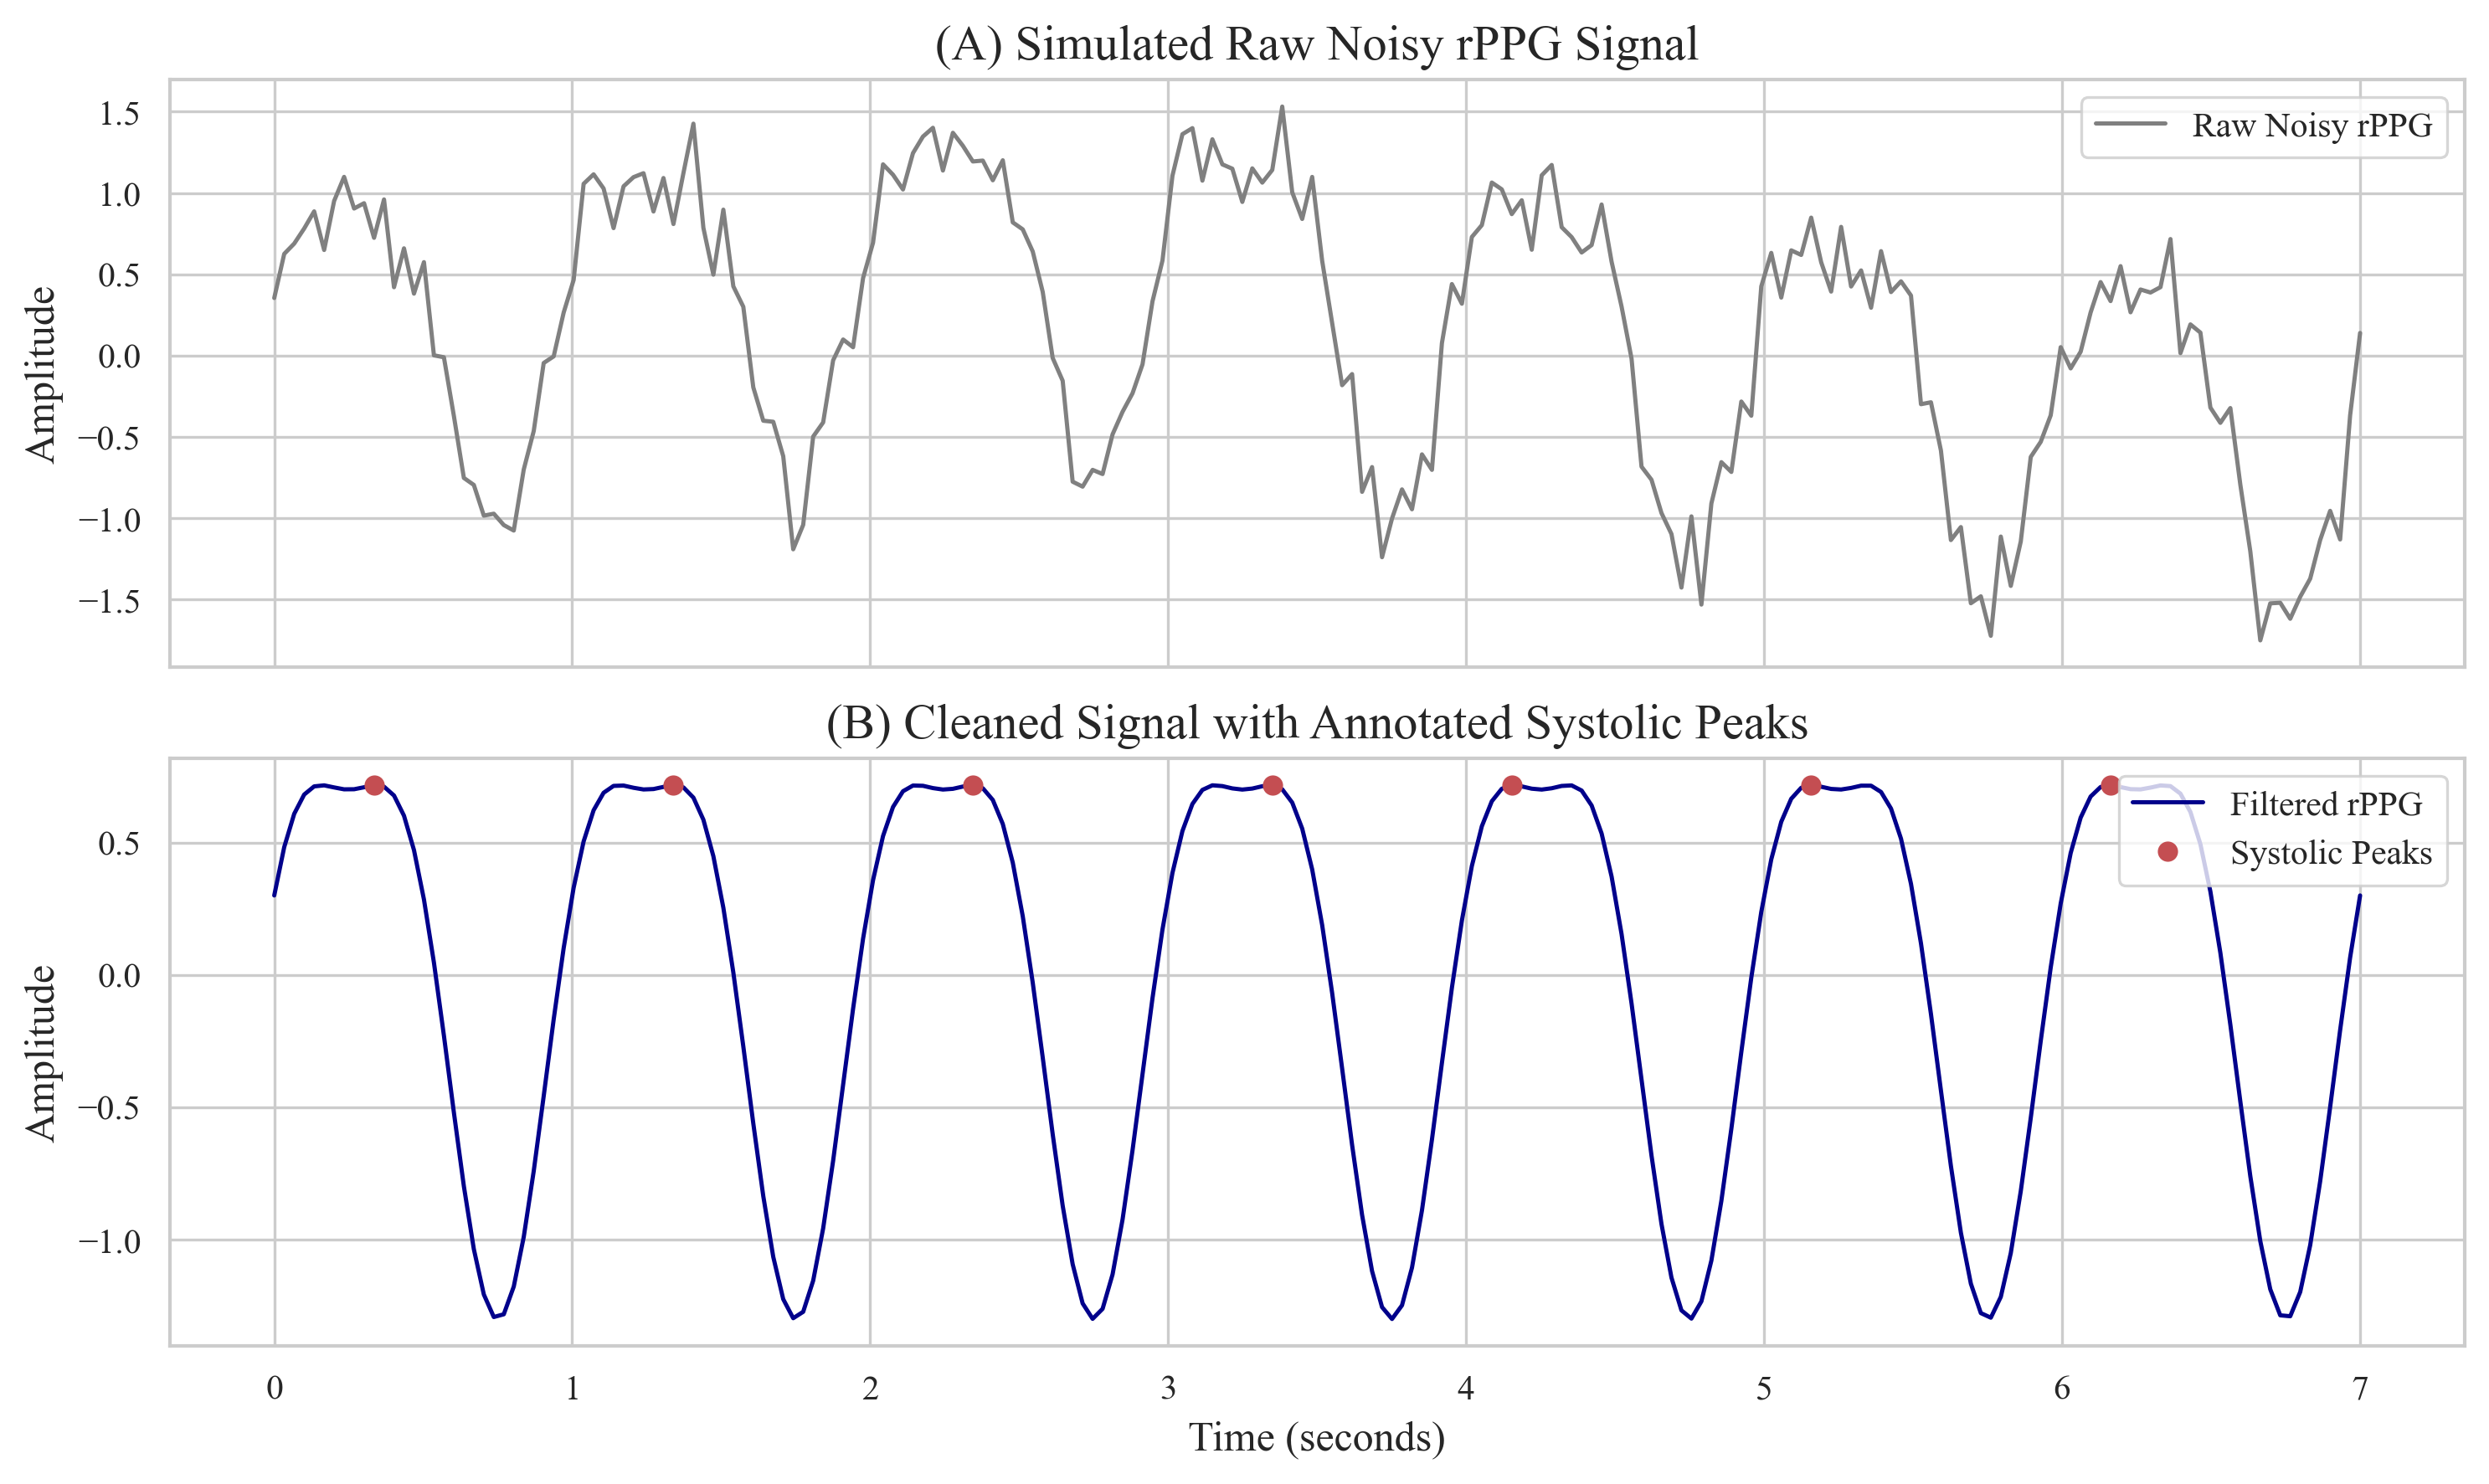
\includegraphics[width=\linewidth]{results/figures/fig2_signal_processing.png}
\caption{Multi-Stage Signal Conditioning: Demonstrating the isolation of the BVP waveform and the morphological preservation achieved by the Savitzky-Golay filter.}
\label{fig:sigproc}
\end{figure}

\subsection{Decoupled Neural Architecture: MODEL-06-SepHead}
The processed 1D Blood Volume Pulse (BVP) is fed into \textbf{MODEL-06-SepHead}. This network is designed to solve the physiological gradient conflict between SBP and DBP estimation. 

\begin{figure}[ht]
\centering
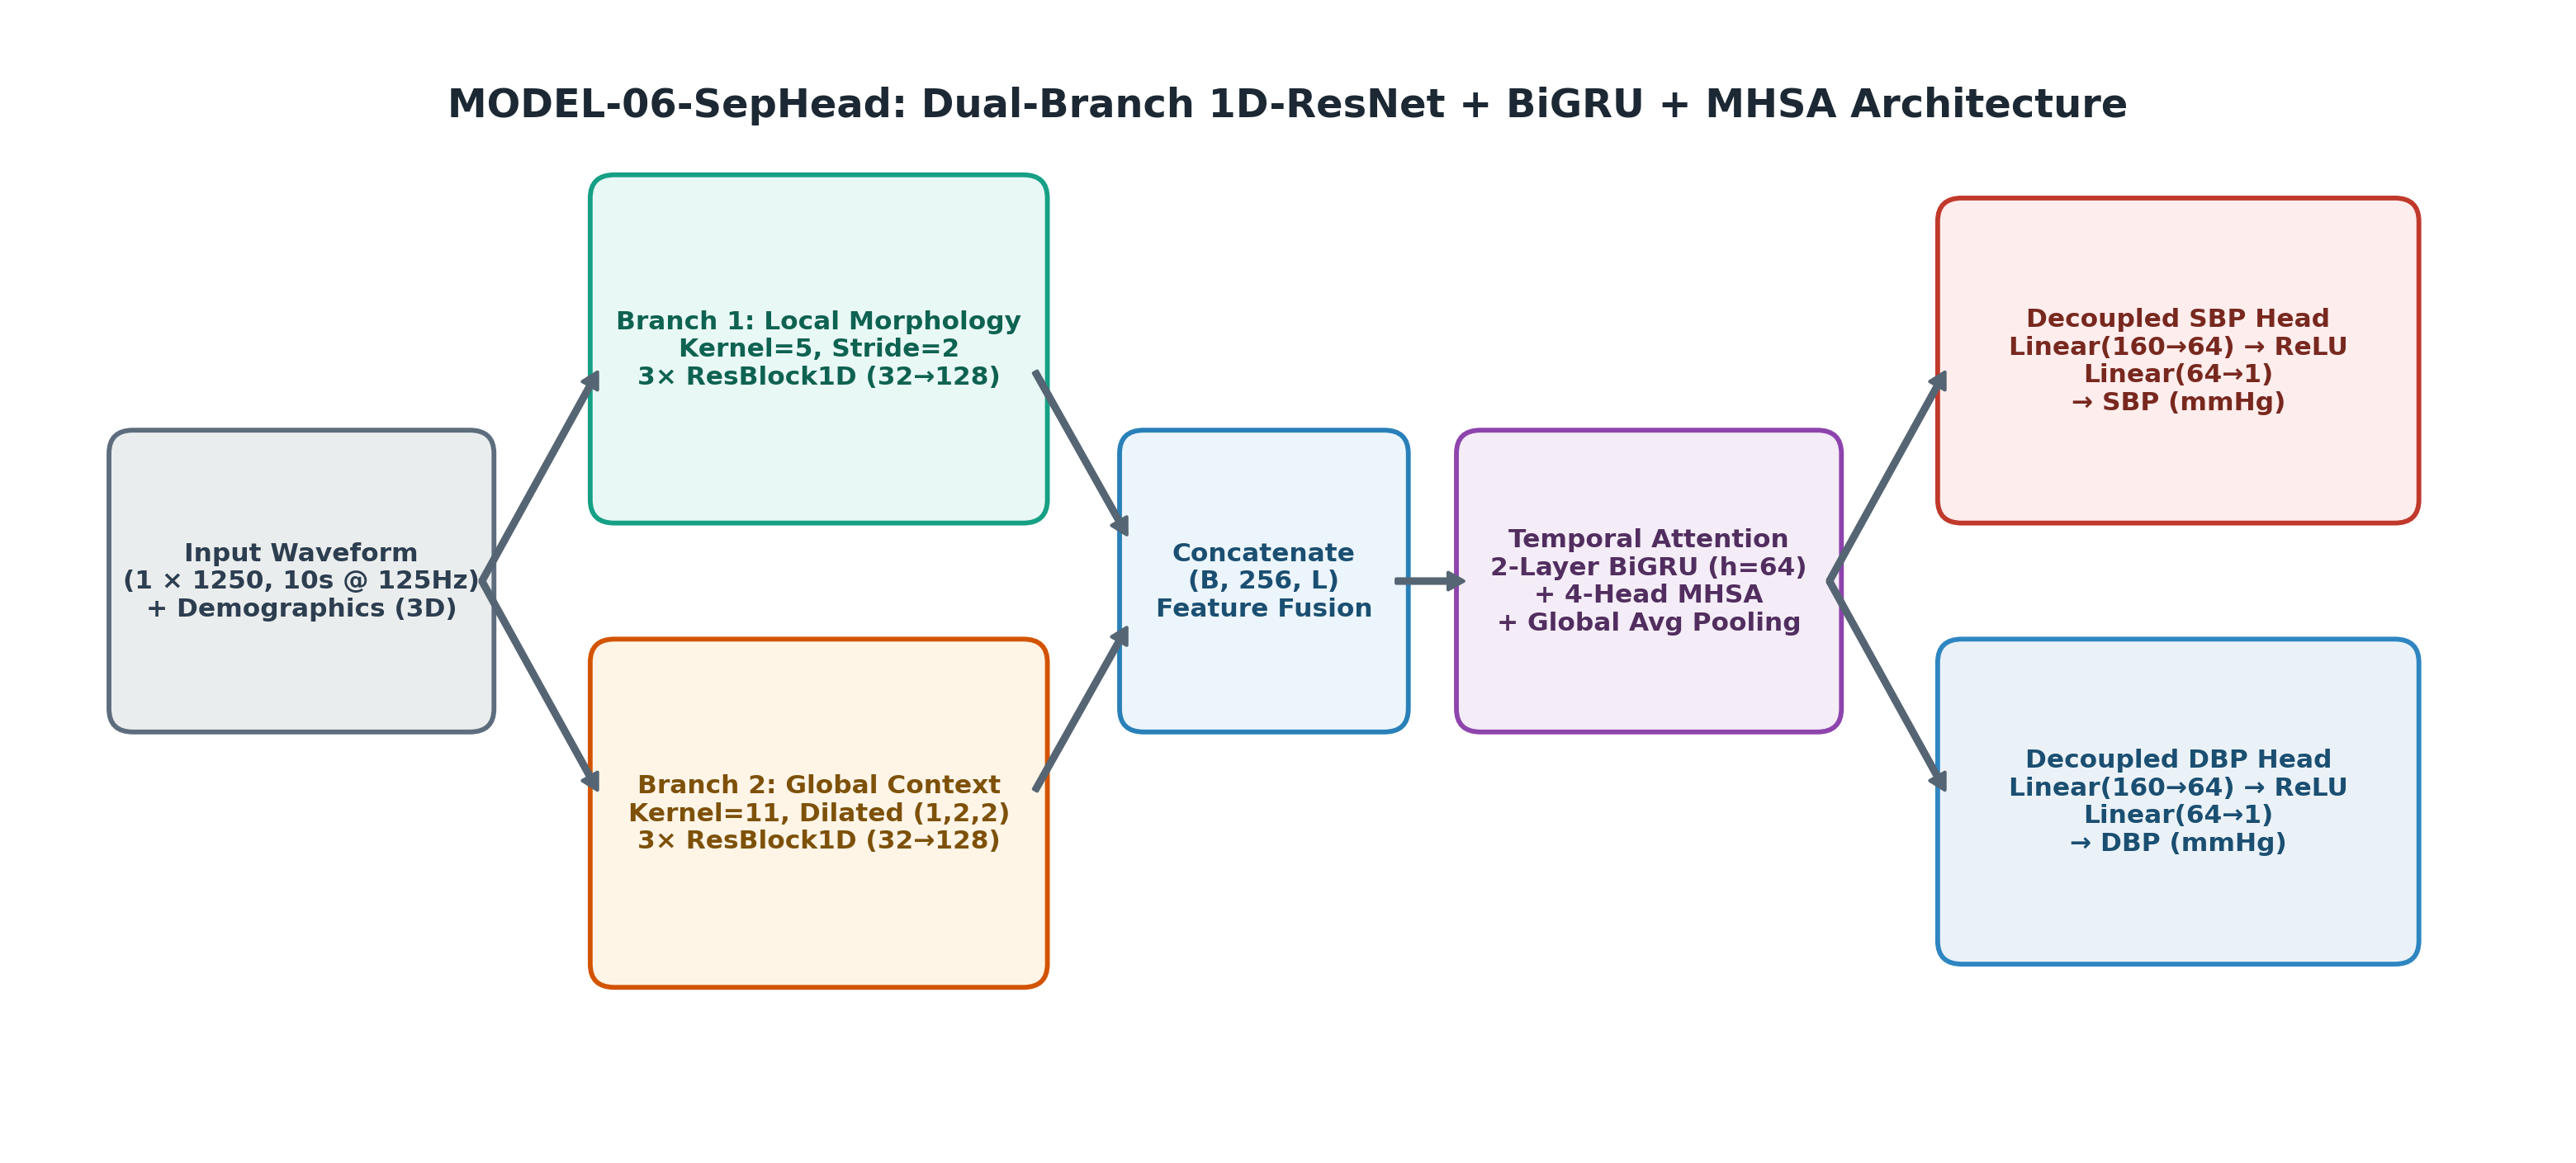
\includegraphics[width=\linewidth]{results/figures/fig_model06_architecture.png}
\caption{MODEL-06-SepHead Architecture: The shared temporal sequence representation is routed into distinct, mathematically decoupled dense heads for SBP and DBP regression.}
\label{fig:model06}
\end{figure}

First, a Multi-Scale 1D-ResNet backbone extracts both local transient features and wide receptive field features using dilated convolutions. The sequence is then modeled by a Bidirectional Gated Recurrent Unit (BiGRU) and augmented with Multi-Head Self-Attention (MHSA):
\begin{equation}
\text{Attention}(Q, K, V) = \text{softmax}\left(\frac{QK^T}{\sqrt{d_k}}\right) \cdot V
\end{equation}
Finally, the latent representations are processed by two completely decoupled regression heads, trained using independent Mean Squared Error (MSE) loss, to predict SBP and DBP.
